\section{案例一：CVE-2022-24768内部权限问题}

\subsection{漏洞详解与复现}

\textbf{（1）漏洞背景}

Argo CD 是 Kubernetes 生态中广泛使用的声明式 GitOps 持续交付工具。其典型部署形态为：Argo CD 控制平面以相对高权限身份（对集群资源拥有创建/更新/删除能力）持续对齐 Git 仓库中的“期望状态”。
该架构提升交付一致性的同时，也带来显著的安全挑战：一旦普通用户能够影响 Argo CD 的控制决策，便可能借助控制平面权限实现权限边界放大。

\textbf{CVE 描述}：CVE-2022-24768 为 Argo CD 的不当访问控制（Improper Access Control）漏洞。\textbf{所有未修复版本}（自 1.0.0 起）均存在风险，0.5.x 与 0.8.x 系列中包含该问题的受限版本。攻击者需要满足以下前置条件之一：
（i）对某个 Application 的源 Git/Helm 仓库具备 push 权限；或（ii）在 Argo CD 中对该 Application 具备 \texttt{sync} 与 \texttt{override} 权限。满足条件后，攻击者可通过构造/修改仓库内容或应用配置，诱导 Argo CD 以其控制平面权限执行超出攻击者原始 RBAC 边界的操作，进而\textbf{潜在提升至 admin 级别能力}。官方已在 Argo CD \textbf{2.1.14、2.2.8、2.3.2} 中发布补丁。\textbf{缓解措施可降低风险但不能替代升级}。

\textbf{主要成因分类}：安全逻辑缺陷 / 访问控制缺陷（已授权用户的权限放大）。
\textbf{攻击链条描述}：其抽象攻击链可概括为：
\begin{enumerate}
        \item \textbf{合法身份阶段}：攻击者以普通 Argo CD 用户身份登录；
        \item \textbf{配置影响阶段}：凭借对 Application 的 \texttt{sync+override} 或对源码仓库的 push 权限，注入恶意资源清单；
        \item \textbf{控制平面滥用阶段}：Argo CD 按 GitOps 同步逻辑将恶意资源应用到集群；
        \item \textbf{权限提升阶段}：借助被创建的高权限 RBAC 绑定（如 \texttt{ClusterRoleBinding}）获得集群级管理员能力。
\end{enumerate}
\textbf{（2）漏洞复现}

本节给出可复现的实验流程：通过构造一个包含“正常资源 + 恶意 RBAC 绑定”的 Git 仓库，并为低权用户配置 \texttt{sync+override} 权限，使其能够触发 Argo CD 同步，从而在集群中创建管理员级绑定实现提权。

\textbf{环境配置}：
\begin{itemize}
        \item Kubernetes 版本：vX.Y.Z（\texttt{kind}/\texttt{minikube} 均可，本文复现以可部署 Argo CD 的版本为准，具体版本号以实验环境为准）；
        \item 受影响组件：Argo CD v2.3.1（漏洞版本，补丁版本为 2.3.2/2.2.8/2.1.14）；
        \item 测试负载：
\begin{itemize}
        \item Git 仓库：\url{https://github.com/Ivanbeethoven/bad_repo}；
        \item 其中包含 \texttt{app.yaml}（正常资源，如 nginx）与 \texttt{hack-admin.yaml}（恶意 \texttt{ClusterRoleBinding}，将用户 \texttt{bob} 绑定到管理员角色）。
\end{itemize}
\end{itemize}

\textbf{攻击步骤}：

本文复现按“部署漏洞版本\,$\rightarrow$\,创建宽松 AppProject\,$\rightarrow$\,授予低权用户 \texttt{sync+override}\,$\rightarrow$\,创建指向恶意仓库的 Application\,$\rightarrow$\,触发同步\,$\rightarrow$\,验证权限变化”的流程进行。
为避免正文过长，关键命令与清单见附录\ref{app:cve-2022-24768}。


\textbf{攻击结果}：综合上述验证，可观察到“权限边界放大”的典型迹象：
\begin{itemize}
        \item 低权用户 bob 原本仅被授予 \texttt{applications sync/override}（对特定项目范围内应用）；
        \item 通过影响 Git 期望状态或应用同步动作，最终间接在集群中创建了高权限 RBAC 绑定；
        \item 其效果表现为 \texttt{kubectl auth can-i '*' '*'} 在 \texttt{--as bob} 条件下返回 \texttt{yes}。
\end{itemize}
\begin{figure}[htbp]
        \centering
        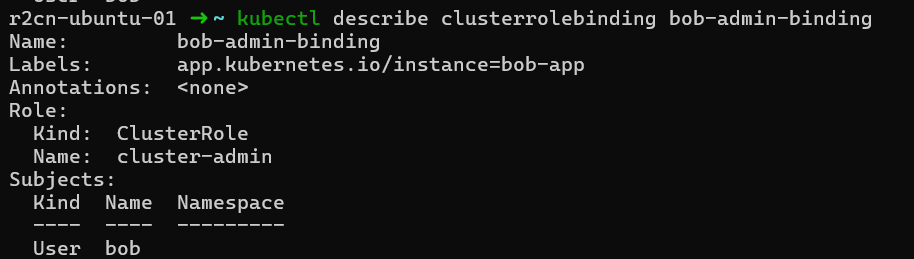
\includegraphics[width=1\textwidth]{images/cve1/image2.png}
        \caption{漏洞复现实验结果示意（验证权限变化）}
        \label{fig:cve-2022-24768-poc}
\end{figure}

\begin{figure}[htbp]
        \centering
        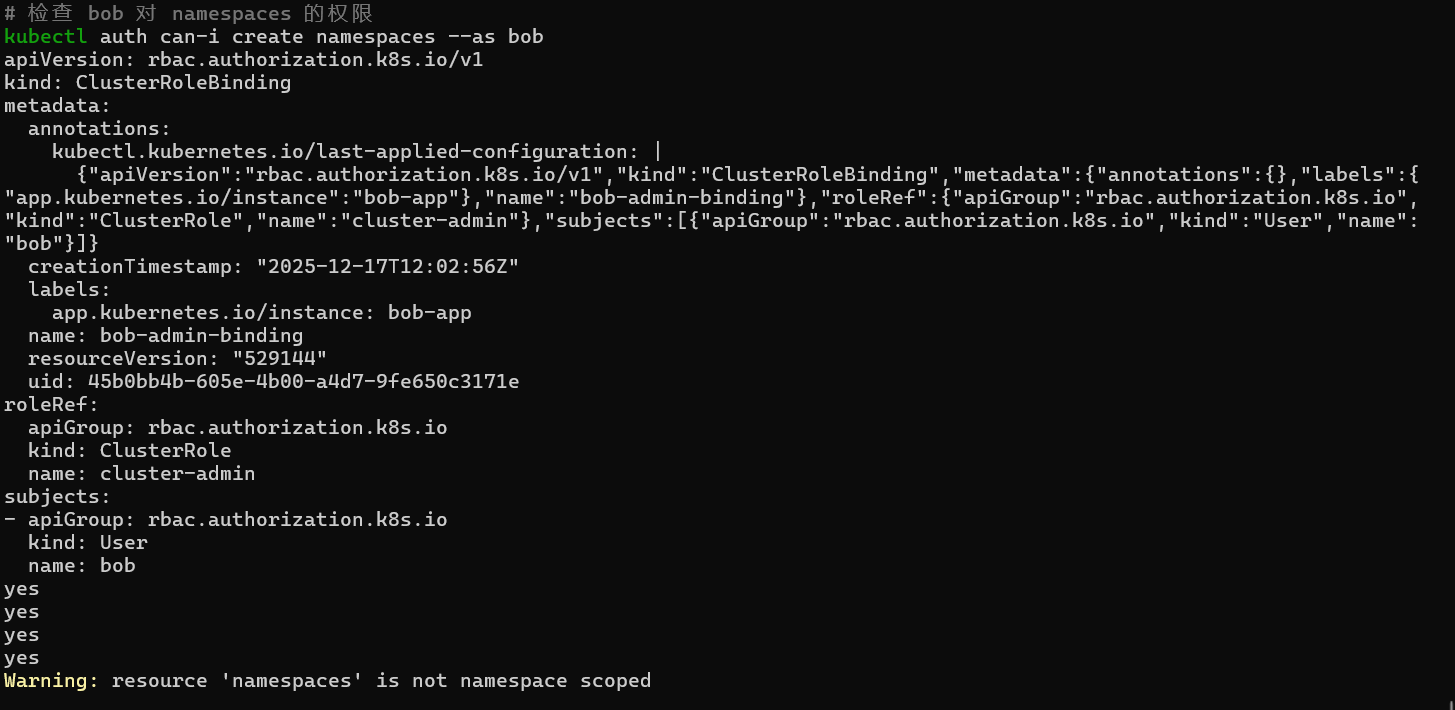
\includegraphics[width=1\textwidth]{images/cve1/image1.png}
        \caption{漏洞复现实验结果示意（验证是否有命令空间级别权限）}
        \label{fig:cve-2022-24768-chain}
\end{figure}

\subsection{策略部署}
使用本文方法生成的最佳安全策略如下（经多智能体评估体系选出）。该策略遵循“纵深防御（Defense in Depth）”，强调\textbf{限制配置可达性、限制配置表达力、限制权限来源}，并将“升级补丁”作为必要但非唯一手段。

\textbf{策略概述}：
\begin{itemize}
        \item \textbf{防控层次（layer）}：身份与权限 / 策略执行 / 准入控制 / 审计与治理
        \item \textbf{防控方法（method）}：Kubernetes RBAC 收敛 + Argo CD RBAC 加固 + 准入控制校验 AppProject/权限策略 + 身份组映射白名单 + 审计告警 + 基线与回滚 + 分阶段强制
        \item \textbf{使用工具}：Kubernetes RBAC、Argo CD RBAC（Casbin）、OPA/Gatekeeper（或 Kyverno）、Kubernetes Audit（以及 SIEM/告警系统）
\end{itemize}

\textbf{策略配置}：为便于复用与自动化，以下给出关键配置片段（可按“先审计、后强制”的方式分阶段落地）。

\begin{itemize}
        \item \textbf{Kubernetes RBAC（集群层）}：收敛 \texttt{AppProject} 的创建/更新/删除权限，仅平台管理员可写；
        \item \textbf{Argo CD RBAC（应用层）}：\texttt{policy.default=role:readonly}，并显式隔离 \texttt{projects/repositories/clusters/exec} 等高风险能力；
        \item \textbf{准入控制（策略层）}：在 \texttt{AppProject} 创建/更新时校验策略表达，禁止通配符放权、强制项目域前缀、禁止授予高危资源写权限；
        \item \textbf{审计与基线（治理层）}：将关键配置纳入 Git 基线与审计告警，降低权限漂移风险。
\end{itemize}

为避免正文堆叠大量 YAML/Rego 清单，Kubernetes RBAC、Argo CD RBAC、Gatekeeper/Kyverno 准入策略的完整可用代码与应用命令见附录\ref{app:cve-2022-24768}。

\subsection{三因素分析}

\textbf{（1）有效性（Effectiveness）}
该策略在攻击链的多个关键点形成“多点阻断”：
\begin{itemize}
        \item Kubernetes RBAC 限制 \texttt{AppProject} 写入，降低“放开 sourceRepos/destinations/whitelist”导致的爆炸半径；
        \item Argo CD RBAC 默认只读并隔离高危资源写权限，使低权用户难以获得可用于放大控制面的关键操作集合；
        \item 准入控制对策略表达施加硬约束，防止隐蔽通配符放权与权限漂移；
        \item 身份治理约束授权来源，降低组注入或错误映射造成的隐式提权。
\end{itemize}
在复现实验中，若上述策略生效，则攻击者即使拥有 \texttt{sync} 权限，也难以通过修改 AppProject/仓库/策略来诱导 Argo CD 创建集群级高权限绑定，攻击路径被显著收敛。

\textbf{（2）无干扰性（Interference）}
该策略以“最小必要变更”为原则，主要影响集中在管理面与配置流程：
\begin{itemize}
        \item 对业务同步的直接影响可控：保留项目内正常的 \texttt{sync} 能力，仅收紧 \texttt{override}、高危资源写权限与危险策略表达；
        \item 准入控制建议先 audit 再 enforce，可显著降低误拦截对业务的冲击；
        \item 额外运维开销主要来自 RBAC 精细化与准入规则维护，但可通过模板化与 GitOps 基线降低长期成本。
\end{itemize}

\textbf{（3）可部署性（Deployability）}
该策略依赖的能力均为云原生常用组件，具有较强可落地性：
\begin{itemize}
        \item Kubernetes RBAC 与 Argo CD RBAC 为原生能力，配置可版本化并可审计；
        \item Gatekeeper/Kyverno 为成熟的准入控制方案，可按项目逐步推广；
\end{itemize}

